\documentclass[../thesis.tex]{subfiles}
\begin{document}

\chapter{Theory}
\label{chp:theory}

Within this chapter the theory needed to solve a CFD case is shown.

\section{Computational Fluid Dynamics}

Computational fluid dynamics or CFD in short is the computer based solving of problems regarding fluid flow, heat transfer, chemical reactions or other phenomena. The concept is used in a large variety of applications within the fields of engineering and science for at least the last 60 years \cite{versteeg2007introduction}.

Within \autoref{fig:cdf_procedure} the general procedure of solving a CFD case is shown.
\begin{figure}[htbp]
	\centering
	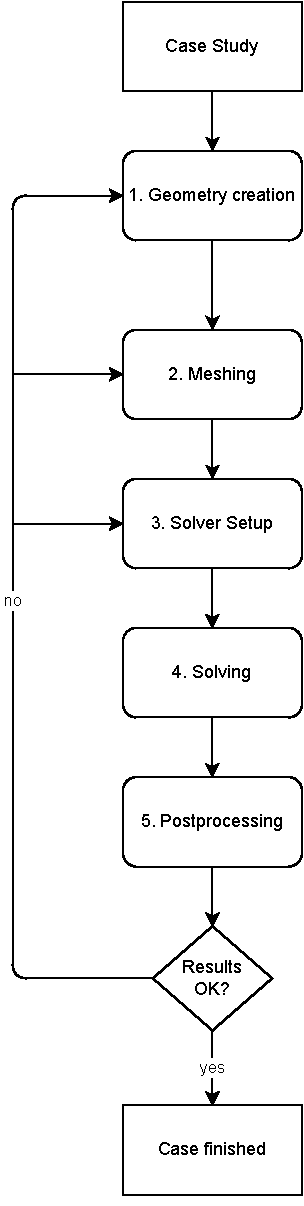
\includegraphics[scale=1.0]{CFD_general}
	\caption{CFD Case Procedure}
	\label{fig:cdf_procedure}
\end{figure}

The first step is to model the domain's geometry. In case of Ansys this step can either be done within the CFD software itself or an external CAD program. After the geometry is created or imported form an external source a mesh needs to be created. This mesh is the basis for the solver to solve the case and a vary important step. The way the mesh is set up has a significant influence on the model's results and the computational resources needed. The finer the mesh the more computational power is needed. By lowering the grid's element size the resources needed or simulation time increases exponentially.

When meshing is finished the solver has to be configured. Setting up the governing equations, simulation time and boundary conditions are steps that need to be done here for example. The hole setup is described in greater detail within \autoref{chp:model}. After the solver setup the case can be run by starting the solver. Depending on the resources needed or available this step can need some further configuration.

When the solving process has come to an end the results can be inspected. If they contain errors some of the previous done steps need to be redone and adapted. 

All in all solving a CFD case is an iterative process that needs to be gone through until the results look as expected and can be trusted. Further details are given in \autoref{chp:model} and \autoref{chp:limitations}.

\section{Navier-Stokes-Equations}

In this thesis the chemical reaction diffusion advection front within a radial reactor is solved using Ansys FLUENT witch solves the incompressible Navier-Stokes Equations (\autoref{eqn:Navier-x} - \autoref{eqn:Navier-z})

\begin{equation}
	\label{eqn:Navier-x}
	\begin{aligned}
	\rho \dfrac{Du}{Dt} = - \dfrac{\partial p}{\partial x}
		& + \dfrac{\partial}{\partial x} \left[
				2 \mu \cdot \dfrac{\partial u}{\partial x} + \lambda \mathrm{div}(\bold{u})
			\right] \\
		& + \dfrac{\partial}{\partial y} \left[
		 \mu  \left( \dfrac{\partial u}{\partial y} + \dfrac{\partial v}{\partial x} \right)
		\right] \\
		& + \dfrac{\partial}{\partial z} \left[
		\mu  \left( \dfrac{\partial u}{\partial z} + \dfrac{\partial w}{\partial x} \right)
		\right] +
		S_{Mx}
	\end{aligned}
\end{equation}

\begin{equation}
	\label{eqn:Navier-y}
	\begin{aligned}
		\rho \dfrac{Dv}{Dt} = - \dfrac{\partial p}{\partial y}
		& + \dfrac{\partial}{\partial x} \left[
		\mu  \left( \dfrac{\partial u}{\partial y} + \dfrac{\partial v}{\partial x} \right)
		\right] \\
		& + \dfrac{\partial}{\partial y} \left[
		2 \mu \cdot \dfrac{\partial v}{\partial y} + \lambda \mathrm{div}(\bold{u})
		\right] \\
		& + \dfrac{\partial}{\partial z} \left[
		\mu  \left( \dfrac{\partial v}{\partial z} + \dfrac{\partial w}{\partial y} \right)
		\right] +
		S_{My}
	\end{aligned}
\end{equation}

\begin{equation}
	\label{eqn:Navier-z}
	\begin{aligned}
		\rho \dfrac{Dw}{Dt} = - \dfrac{\partial p}{\partial z}
		& + \dfrac{\partial}{\partial x} \left[
		\mu  \left( \dfrac{\partial u}{\partial z} + \dfrac{\partial w}{\partial x} \right)
		\right] \\
		& + \dfrac{\partial}{\partial y} \left[
		\mu  \left( \dfrac{\partial v}{\partial z} + \dfrac{\partial w}{\partial y} \right)
		\right] \\
		& + \dfrac{\partial}{\partial z} \left[
		2 \mu \cdot \dfrac{\partial w}{\partial z} + \lambda \mathrm{div}(\bold{u})
		\right] +
		S_{Mz}
	\end{aligned}
\end{equation}

in addition to the incompressible continuity equation.

\begin{equation}
	\label{eqn:continuity}
	\mathrm{div}(\bold{u}) = 0
\end{equation}

These four equations form a system of non-linear partial differential equations. These have to be solved numerically because there is no analytical solution to this problem including it's boundary conditions. The solution is generated by splitting the domain into small elements and solving the set of equations for each element to obtain a solution for the hole geometry. This method known as Finite Volume Method is described in greater detail within the following section.

\section{Finite Volume Method}

The finite Volume Method is a discretization method. It converts the set of partial differential equations into a system of linear algebraic equations \cite{darwish2021finite}. This is done in two steps. At first the partial differential equations are integrated and so transformed into balance equations \cite{darwish2021finite}. 

\subsection{Semi-Discretization}

For demonstration the conservation equation for a generic variable $ \Phi $ is given by

\begin{equation}
	\label{eqn:conserv_eq}
	\underbrace{\dfrac{\partial(\rho \Phi)}{\partial t}}_{\text{transient term}} + \underbrace{\nabla \cdot (\rho \bold{u} \Phi)}_{\text{convective term}} = \underbrace{\nabla \cdot (\Gamma_\Phi \nabla \Phi)}_{\text{diffusion term}} + \underbrace{S_\Phi}_{\text{source term}}
\end{equation}

Within this equation $ \rho $ represents the density and $ \bold{u} $ is the velocity vector. $ \nabla $ contains the spacial derivatives and $ \Gamma_\Phi $ is the diffusion coefficient of the property $ \Phi $.
For an easier explanation of the maths behind the method the steady state form of \autoref{eqn:conserv_eq} is used.

\begin{equation}
	\nabla \cdot (\rho \bold{u} \Phi) = \nabla \cdot (\Gamma_\Phi \nabla \Phi) + S_\Phi
\end{equation}

As already stated this equation is integrated over the control volume shown in \autoref{fig:FVM_CV} witch leads to \autoref{eqn:FVM_volint}.

\begin{equation}
	\label{eqn:FVM_volint}
	\int_{V_C} \nabla \cdot (\rho \bold{u} \Phi) dV = \int_{V_C} \nabla \cdot (\Gamma_\Phi \nabla \Phi) dV + \int_{V_C} S_\Phi dV
\end{equation}

The volume integrals, within the convective and diffusive term, can be replaced by surface integrals due to the divergence theorem. That leads to the semi-discretized \autoref{eqn:FVM_Aint}.

\begin{equation}
	\label{eqn:FVM_Aint}
	\oint_{\partial V_C} (\rho \bold{u} \Phi) d\bold{S} = \oint_{\partial V_C} (\Gamma_\Phi \nabla \Phi) d\bold{S} + \int_{V_C} S_\Phi dV
\end{equation}

The variable $ \bold{S}$ is the surface vector, the operator ($\cdot$) is the dot product and $ \oint_{\partial V_C}$ is the surface integral operator.

\subsection{Surface Integration}

As seen in \autoref{eqn:FVM_Aint} surface integrals are needed to calculate the value of the property $\Phi$ for the control volume. Theses surface integrals can be split into a summation over each cell surface. This step can be done for each the convective shown in \autoref{eqn:conv_sint} and the diffusion term shown in \autoref{eqn:diffu_sint}.

\begin{equation}
	\label{eqn:conv_sint}
	\oint_{\partial V_C} (\rho \bold{u} \Phi) d\bold{S} = \sum_{f_i}^{n_{\text{faces}}}\left( \int_{f} (\rho \bold{u} \Phi) d\bold{S} \right)
\end{equation}

\begin{equation}
	\label{eqn:diffu_sint}
	\oint_{\partial V_C} (\Gamma_\Phi \nabla \Phi) d\bold{S} =  \sum_{f_i}^{n_{\text{faces}}}\left( \int_{f} (\Gamma_\Phi \nabla \Phi) \right)
\end{equation} 

\begin{figure}[htbp]
	\centering
	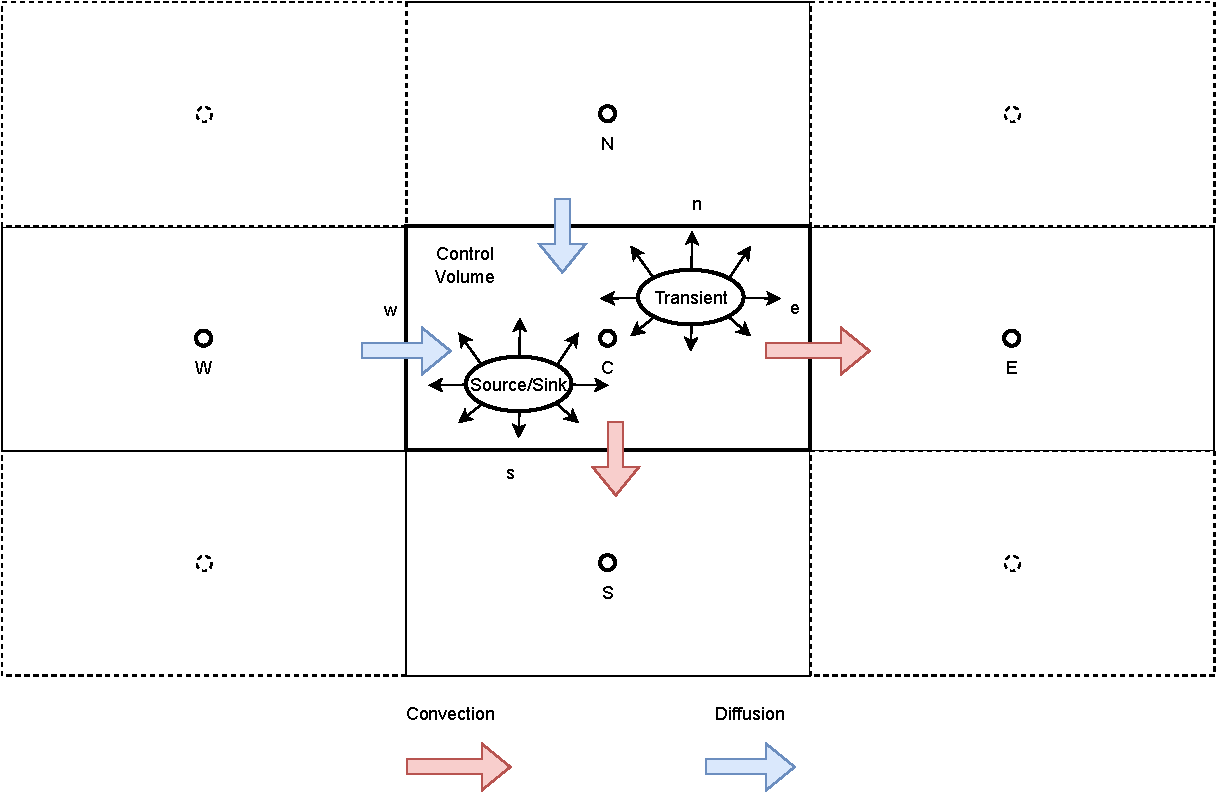
\includegraphics[scale=0.70]{Control_Volumen}
	\caption{Control Volume example}
	\label{fig:FVM_CV}
\end{figure}

\section{Solution Method}

\section{Fluid Phenomena}

\end{document}